\textbf{Beispiel 3}\\ \\
a)\\ \\
Freigeschnittene Blöcke:
\begin{figure}[h]
	\centering
	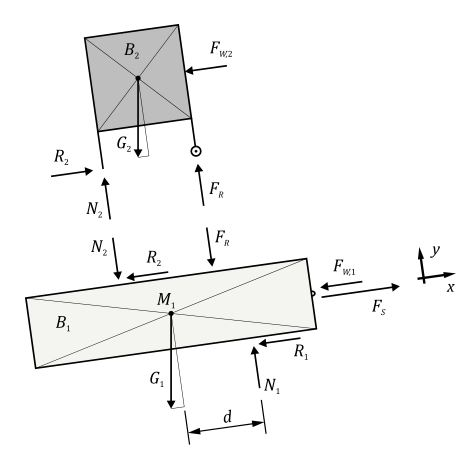
\includegraphics[width= 8cm]{tikz/27_09_2019_3a}
\end{figure}
\newline
Mit den Kräften
\[
	F_{W,2} = C_2v^2 \quad,\quad G_2 = m_2g
\]
Die Gleichgewichtsbedingungen lauten
\begin{align*}
	\textbf{e}_x &: R_2 - G_2\sin(\alpha) - F_{W,2} = 0\\
	\textbf{e}_y &: -G_2\cos(\alpha) + N_2  + F_R= 0 \\
	\textbf{e}_z &: G_2\sin(\alpha)\left(\frac{a_2}{2} + h_2\right) + F_{W,2}\left(\frac{a_2}{2} + h_2\right) + F_Ra_2 - G_2\cos(\alpha)\frac{a_2}{2} = 0
\end{align*}
Aus diesen Gleichungen folgen die anderen gesuchten Kräfte
\begin{align*}
	R_2 &= G_2\sin(\alpha) + F_{W,2} \\
	N_2 &= G_2\cos(\alpha) - F_R
	F_R &= \frac{1}{2}G_2\cos(\alpha) - \frac{1}{a_2}\left(G_2\sin(\alpha) + F_{W,2}\right)\left(\frac{a_2}{2} + h_2\right)
\end{align*}
b)\\ \\
Um die gesuchte Geschwindigkeit zu ermitteln muss $F_R$ bei dieser Geschwindigkeit 0 werden. Daraus folgt
\begin{align*}
	\frac{1}{2}G_2\cos(\alpha) &- \frac{1}{a_2}\left(G_2\sin(\alpha) + F_{W,2}\right)\left(\frac{a_2}{2} + h_2\right) = 0 \\
	\frac{1}{2}G_2\cos(\alpha) &- \frac{1}{a_2}\left(G_2\sin(\alpha) + C_2v^2_{max}\right)\left(\frac{a_2}{2} + h_2\right) = 0 \\
	v_{max} &= \sqrt{\frac{G_2}{C_2}\left(\cos(\alpha)\frac{a_2}{a_2 + 2h_2} - \sin(\alpha)\right)}
\end{align*}
c)\\ \\
Mit dem Ergebnis aus Punkt b) folgt
\begin{align*}
	0 = &\sqrt{\frac{G_2}{C_2}\left(\cos(\alpha_{max})\frac{a_2}{a_2 + 2h_2} - \sin(\alpha_{max})\right)}\\
	\sin(\alpha_{max}) &= \cos(\alpha_{max})\frac{a_2}{a_2 + 2h_2}\\
		\tan(\alpha_{max}) &= \frac{a_2}{a_2 + 2h_2} \\
		\alpha_{max} &= \arctan\left(\frac{a_2}{a_2 + 2h_2}\right)
\end{align*}
Mit der notwendigen Haftbedingung
\[
	R_2 < \mu_A^hN_2
\]
und den beiden Kräften, ermittelt aus den Gleichgewichtsbedingungen
\[
	R_2 = G_2\sin(\alpha_{max}) \quad,\quad N_2 = G_2\cos(\alpha_{max})
\]
folgt schließlich
\[
	\mu_A^h = \tan(\alpha_{max})
\]
d)\\ \\
Die notwendigen Gleichgewichtsbedingungen für B1 lauten
\begin{align*}
	\textbf{e}_x &: F_{W,1} + R_1 + R_2 + G_1\sin(\alpha) - F_S = 0\\
	\textbf{e}_y &: N_2 + F_R + G_1\cos(\alpha) - N_1 = 0\\
	\textbf{e}_z &: N_2\frac{a_2}{2} + R_2\frac{h_1}{2} + N_1d - F_R\frac{a_2}{2} - R_1\frac{h_1}{2} = 0
\end{align*}
\newpage
\noindent
Alle gesuchten Terme werden mit diesen Gleichungen bestimmt und lauten
\begin{align*}
	F_{W,1} &= C_1v^2 \\
	R_1 &= \mu_1^gN_1 \\
	G_1 &= m_1g \\
	F_S &= F_{W,1} + R_1 + R_2 + G_1\sin(\alpha) \\
	N_1 &= N_2 + F_R + G_1\cos(\alpha) \\
	d &= \frac{1}{N_1}\left(\frac{a_2}{2}(F_R - N_2) + \frac{h_2}{2}(R_1 - R_2)\right)
\end{align*}
Die verwendete Zeichnung ist in Punkt a) ersichtlich. \\ \\
